\section{Experiments}
\label{sec:experiments}

We evaluate \framework{} through two research questions: \textbf{RQ1} (Effectiveness and Efficiency): \emph{Can \framework{} learn an effective and efficient KG-RAG policy when trained on a target KG?}; \textbf{RQ2} (Cross-KG Transferability): \emph{Does \framework{} generalize to unseen KGs without additional training?}
For both research questions, we compare against established LLM-only and LLM+KG baselines to assess effectiveness, efficiency, and transferability.

\subsection{Experimental Setup}

\noindent \textbf{Models.}
We use Qwen2.5-3B-it~\citep{qwen2025qwen25technicalreport} as our base model. For the other baseline methods, we use Qwen2.5-7B-it, Qwen2.5-72B-it, Qwen3-235B-A22B-Instruct-2507~\citep{yang2025qwen3}, and Llama2-7B-it (only for the fine-tuned planning in RoG~\citep{Luo2024RoG}), following the setups used in prior work.

\noindent \textbf{Datasets.}
We mainly evaluate \framework{} in-domain on (1) \dataset{WebQSP}~\citep{Yih2016WebQSP}: natural-language questions over Freebase, mostly 1–2 hop questions, using the official 3{,}098/1{,}639 train/test QA split; and (2) \dataset{ComplexWebQuestions (CWQ)}~\citep{Talmor2018CWQ}: compositional, multi-hop questions over Freebase with a 24{,}649/3{,}531 train/test QA split. For scalability, we extract 2-hop subgraphs for each question as in RoG~\citep{Luo2024RoG}. See Appendix~\ref{appendix:datasets} for detailed sources.
We evaluate the plug-and-play approach on diverse KGQA benchmarks spanning two categories of KGs: (1) \emph{Freebase} type---\dataset{SimpleQA}~\citep{bordes2015simplequestions} and \dataset{GrailQA}~\citep{gu2021grailqa}, which share the Freebase KG but differ in question complexity and reasoning path distributions; and (2) \emph{Wikidata} type---\dataset{T-REx}~\citep{elsahar2018trex} and \dataset{QALD-10en}~\citep{usbeck2023qald10} for cross-schema generalization. Appendix~\ref{appendix:datasets} provides a summary of dataset sources, schema, and evaluation splits.

\noindent \textbf{Metrics.} Following prior works~\citep{Luo2024RoG, Sun2024ToG, Chen2024Pog, park2026prograg} to evaluate KGQA performance, we use \textit{Hits@1} (1 if the ground-truth answer appears in the single search, and 0 otherwise). For efficiency, we report \emph{total tokens} and \emph{generated tokens} (completion-only), measured end-to-end per query, aggregated across all turns. 
This serves as a proxy for inference time and compute cost. For fair comparison, all token counts are computed with the Qwen2.5 tokenizer. We also report the \emph{number of modules} to compare workflow complexity, and we analyze single-query latency and batched throughput on a single NVIDIA H100 GPU.


\noindent \textbf{Baselines.}
We compare three classes of approaches: (1) \emph{LLM-only} methods that do not access an external KG: IO~\citep{brown2020gpt3} and Chain-of-Thought (CoT)~\citep{wei2022chain} prompting; (2) \emph{prior KG-augmented} pipelines: \textsc{RoG}~\citep{Luo2024RoG}, which uses a \emph{fine-tuned} modular workflow with LLaMA2-7B-it as the planner and we use the Qwen family as reasoner, and \textsc{ToG}~\citep{Sun2024ToG} and \textsc{ReKnoS}~\citep{Wang2025ReKnoS}, which use a \emph{prompt-based} modular workflow; and (3) our method \framework{}. For LLM-only baselines, we employ LLM-as-Judge~\citep{zheng2023llmasajudge} using gpt-4o-mini~\citep{openai2024gpt4omini} to semantically match predicted answers to ground truth. We report the average and standard deviation over 5 runs for all models and baselines. Full details for the baselines are provided in Appendix~\ref{appendix:baselines}. 

\noindent\textbf{Implementation details.} \label{sec:kg_r1_implementation}
We use VERL~\citep{sheng2024hybridflow} and vLLM-backed decoding~\citep{kwon2023efficient} for implementing the \framework{} agent. Training uses distributed optimization with gradient checkpointing and offloading. Unless stated otherwise, we set \(H=5\) as the maximum number of turns and \(N=16\) rollouts per query. %
Additional implementation details (e.g., hyperparameters) are provided in Appendix~\ref{appendix:implementation_details}.

\begin{wrapfigure}{t}{.5\textwidth}
  \vspace{-4em}
  \centering
  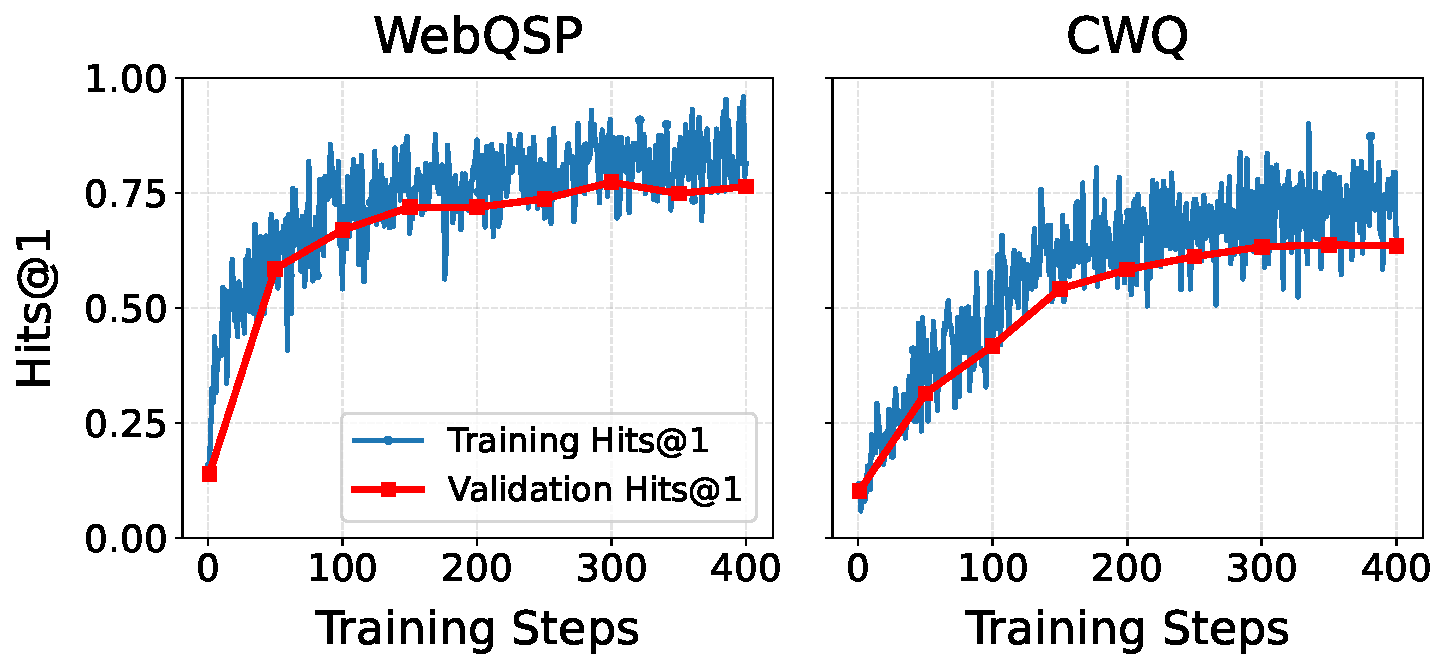
\includegraphics[width=\linewidth]{Figures/hits1_train_vs_validation.pdf}
  \captionof{figure}{Hits@1 over \framework{} training on \dataset{WebQSP} and \dataset{CWQ} for Qwen2.5-3B-it. %
  }
  \label{fig:training_main}
  \vspace{-2em}
\end{wrapfigure}
\subsection{Training Stability and Effectiveness}
Figure~\ref{fig:training_main} shows steady improvements in Hits@1 that gradually plateau as training converges for \framework{} on both \dataset{WebQSP} and \dataset{CWQ}. The validation Hits@1 closely follows the training curve, indicating that the learned policy generalizes well to unseen data in the validation set without significant overfitting. Overall, \framework{} training achieves stable and consistent gains in end-to-end KG-RAG performance.



\subsection{RQ1: Effectiveness and Efficiency Results}
\label{sec:exp1}


\definecolor{first}{RGB}{237, 106, 89}
\definecolor{second}{RGB}{255, 192, 0}
\definecolor{third}{RGB}{91, 155, 213}
\newcommand{\res}[2]{#1\textsubscript{ $\pm$ #2}}
\newcommand{\fir}[2]{\textcolor{first}{\textbf{#1\textsubscript{$\pm$#2}}}}
\newcommand{\sed}[2]{\underline{#1\textsubscript{ $\pm$ #2}}}
\newcommand{\thi}[2]{{#1\textsubscript{ $\pm$ #2}}}
\newcommand{\firi}[1]{\textcolor{first}{\textbf{#1}}}
\newcommand{\seci}[1]{\underline{#1}}
\newcommand{\thii}[1]{{#1}}
\newcommand{\colorres}[3]{\textcolor{#1}{\textbf{#2} \textsubscript{$\pm$ \textbf{#3}}}}

\begin{table*}[!t]
\caption{Performance and efficiency comparison of KGQA methods on WebQSP and CWQ datasets. The maximum turn number is set to $H=5$. All scores are percentages.}
\label{tab:webqsp_cwq_performance_efficiency_comparison_colored}
\vspace{-0.5em}
\begin{center}
\renewcommand{\arraystretch}{1.05}
\small
\resizebox{\textwidth}{!}{%
\begin{tabularx}{1.08\textwidth}{c@{\hspace{0.2em}}c@{\hspace{0.6em}}c@{\hspace{0.2em}}c@{\hspace{0.6em}}c@{\hspace{0.5em}}c@{\hspace{0.5em}}c@{\hspace{0.5em}}c@{\hspace{0.5em}}c}
\toprule
& \multicolumn{2}{c}{\thead{\normalsize Datasets $\rightarrow$}} & \multicolumn{3}{c}{\dataset{WebQSP}} &  \multicolumn{3}{c}{\dataset{CWQ}}
\\
\cmidrule(lr){4-6} \cmidrule(lr){7-9}
& \thead{\normalsize Methods} & \thead{Modules}
& \thead{Hits@1 (\%)} & \thead{Total Tokens} & \thead{Gen Tokens}
& \thead{Hits@1 (\%)} & \thead{Total Tokens} & \thead{Gen Tokens}
\\
\midrule
\multirow{8}{*}{\rotatebox{90}{Qwen 2.5-7B}}
& {IO} & 1
& \res{21.37}{0.07} & \res{151.59}{0.03} & \res{9.29}{0.03}
& \res{16.63}{0.01} & \res{159.76}{0.01} & \res{8.57}{0.01}
\\
& {CoT} & 1
& \res{17.27}{0.09} & \res{260.43}{0.02} & \res{49.13}{0.02}
& \res{14.95}{0.02} & \res{292.46}{0.01} & \res{72.27}{0.01}
\\
& {SC} & 1
& \res{19.26}{0.19} & \res{2098.01}{0.92} & \res{407.60}{0.92}
& \res{17.63}{0.17} & \res{2364.62}{1.24} & \res{603.13}{1.24}
\\
\cmidrule(lr){2-9}
& {RoG} & 2
& \res{79.89}{0.35} & \res{814.61}{0.70} & \res{246.95}{0.67}
& \res{46.32}{0.49} & \res{1219.72}{0.61} & \res{259.46}{0.58}
\\
& {ToG} & 4
& \res{65.00}{4.63} & \res{6455.04}{753.60} & \res{941.52}{109.27}
& \res{32.25}{0.43} & \res{8396.80}{87.06} & \res{1358.54}{17.24}
\\
& {PoG} & 5
& \res{64.81}{0.84} & \res{4474.30}{91.92} & \res{241.14}{5.17}
& \res{32.00}{2.53} & \res{8293.67}{1454.76} & \res{369.84}{45.59}
\\
& {ReknoS} & 3
& \res{61.22}{5.46} & \res{2822.34}{209.87} & \res{558.43}{45.52}
& \res{53.45}{3.03} & \res{2908.55}{222.47} & \res{602.08}{39.33}
\\
\midrule
\multirow{8}{*}{\rotatebox{90}{Qwen 2.5-72B}}
& {IO} & 1
& \res{24.66}{0.07} & \res{153.50}{0.02} & \res{11.20}{0.02}
& \res{22.20}{0.02} & \res{162.04}{0.03} & \res{10.85}{0.03}
\\
& {CoT} & 1
& \res{21.84}{0.04} & \res{271.46}{0.02} & \res{60.16}{0.02}
& \res{22.92}{0.04} & \res{296.81}{0.04} & \res{76.62}{0.04}
\\
& {SC} & 1
& \res{22.62}{0.07} & \res{2177.75}{1.23} & \res{487.34}{1.23}
& \res{24.76}{0.27} & \res{2385.73}{0.51} & \res{624.24}{0.51}
\\
\cmidrule(lr){2-9}
& {RoG} & 2
& \res{81.63}{3.33} & \res{812.32}{7.81} & \res{244.53}{7.79}
& \res{45.05}{2.87} & \res{1205.48}{2.51} & \res{245.34}{2.51}
\\
& {ToG} & 4
& \res{74.47}{0.25} & \res{6810.27}{39.73} & \res{942.91}{5.80}
& \res{43.18}{1.02} & \res{9024.77}{271.68} & \res{1358.32}{41.02}
\\
& {PoG} & 5
& \res{72.88}{6.57} & \res{4759.10}{210.29} & \res{316.25}{16.85}
& \res{43.62}{1.38} & \res{7969.21}{1631.58} & \res{503.29}{116.35}
\\
& {ReknoS} & 3
& \res{75.23}{9.25} & \res{2472.90}{115.94} & \res{488.44}{39.87}
& \res{60.88}{2.54} & \res{2278.71}{196.08} & \res{548.52}{27.79}
\\
\midrule
\multirow{8}{*}{\rotatebox{90}{Qwen 3-235B}}
& {IO} & 1
& \res{24.01}{0.18} & \res{136.05}{0.06} & \res{14.75}{0.06}
& \res{20.22}{0.09} & \res{147.36}{0.16} & \res{17.17}{0.16}
\\
& {CoT} & 1
& \res{26.94}{0.22} & \res{274.66}{0.32} & \res{84.36}{0.32}
& \res{24.38}{0.33} & \res{317.42}{0.31} & \res{118.23}{0.31}
\\
& {SC} & 1
& \res{27.60}{0.15} & \res{2200.20}{1.26} & \res{677.79}{1.26}
& \res{26.13}{0.23} & \res{2551.71}{0.78} & \res{958.22}{0.78}
\\
\cmidrule(lr){2-9}
& {RoG} & 2
& \res{81.68}{0.24} & \res{960.58}{5.90} & \res{254.31}{0.11}
& \res{48.94}{0.39} & \res{1217.51}{10.26} & \res{252.45}{5.18}
\\
& {ToG} & 4
& \res{75.67}{0.37} & \res{6831.66}{28.39} & \res{996.12}{5.21}
& \res{39.82}{0.73} & \res{5389.00}{33.01} & \res{802.97}{9.84}
\\
& {PoG} & 5
& \res{79.13}{1.89} & \res{6818.26}{908.76} & \res{418.26}{49.36}
& \res{44.69}{0.27} & \res{10177.37}{1859.27} & \res{548.77}{82.56}
\\
& {ReknoS} & 3
& \res{84.73}{1.78} & \res{2795.53}{139.20} & \res{592.38}{4.18}
& \res{65.63}{4.86} & \res{2677.92}{281.97} & \res{684.38}{14.06}
\\
\midrule
\oursrow
& \thead{\textbf{\framework{} \scriptsize{(Ours)}}\\\scriptsize{Qwen2.5-3B}} & 1
& \res{82.75}{0.04} & \res{3237.17}{30.34} & \res{308.67}{0.56}
& \res{65.31}{0.14} & \res{3205.95}{42.34} & \res{311.14}{0.52}
\\
\bottomrule
\end{tabularx}
}
\vspace{-1.5em}
\end{center}
\end{table*}


\noindent \textbf{\framework{} demonstrates strong accuracy on trained KGs.}
Table~\ref{tab:webqsp_cwq_performance_efficiency_comparison_colored} reports Hits@1 and token efficiency on \dataset{WebQSP} and \dataset{CWQ}. Despite being trained from a lightweight Qwen2.5-3B base model, \framework{} achieves the strongest overall performance among all compared methods on \dataset{WebQSP}, reaching a Hits@1 of \textbf{82.75}, outperforming RoG built on Qwen2.5-7B (79.89), Qwen2.5-72B (81.63), and even Qwen3-235B (81.68). It also exceeds or is comparable to stronger multi-module baselines such as ToG (75.67), PoG (79.13), and ReKnoS (84.73) while using a substantially smaller backbone.
On the more compositional \dataset{CWQ}, \framework{} achieves a Hits@1 of \textbf{65.31}, improving over RoG by a large margin across all scales (46.32--48.94), and surpassing ReKnoS built on Qwen2.5-7B (53.45), Qwen2.5-72B (60.88), and Qwen3-235B (55.63). Notably, \framework{} remains highly competitive with ReKnoS built on Qwen3-235B (65.31 vs.\ 65.63 on \dataset{CWQ}), despite using a Qwen2.5-3B backbone that is nearly two orders of magnitude smaller. This highlights that reinforcement learning over structured KG actions can substantially improve reasoning effectiveness beyond what is achievable by model scaling alone.

\noindent \textbf{\framework{} achieves efficient inference with reduced generation cost.}
Table~\ref{tab:webqsp_cwq_performance_efficiency_comparison_colored} also reports total and generated tokens. On \dataset{WebQSP}, \framework{} uses only \textbf{308.67} generation tokens, which is 3.05$\times$ fewer than ToG (941.52) and 1.81$\times$ fewer than ReKnoS (592.38), while achieving higher Hits@1 than ToG and comparable performance to ReKnoS. On \dataset{CWQ}, \framework{} generates \textbf{311.14} tokens, reducing generation cost by 2.58$\times$ compared to ToG (802.97) and 2.20$\times$ compared to ReKnoS (684.38), while achieving comparable answer accuracy to ReKnoS and outperforming ToG. Compared with the most token-efficient KG baseline RoG, \framework{} uses moderately more generation tokens (308.67 vs.\ 254.31 on WebQSP; 311.14 vs.\ 252.45 on CWQ), but delivers substantially higher answer accuracy (+1.07 to +20.26 absolute Hits@1 depending on model scale and dataset). This indicates a favorable effectiveness-efficiency tradeoff: \framework{} preserves competitive token efficiency while substantially improving reasoning quality.

\noindent \textbf{Single-agent design reduces system complexity.} Beyond token efficiency, \framework{} simplifies the KG-RAG pipeline into a single-agent architecture. Prior methods typically require 2--5 modules (e.g., retrieval, planning, verification, and answering), whereas \framework{} performs retrieval and reasoning within a unified policy using only one module. This reduces deployment complexity and avoids error propagation across stages. Despite this simplification, \framework{} remains competitive or superior to multi-module systems across both datasets, showing that structured RL can effectively consolidate KG interaction and reasoning into a lightweight unified agent.

\noindent \textbf{Latency and throughput analysis.} 
On a single NVIDIA H100 GPU, we measure (i) single-query end-to-end latency and (ii) batched throughput. The single-query latency averages \(6.4\pm1.5\) s per question, and the batched throughput reaches \(3.7\) samples per second with a batch size of 64. The results suggest the feasibility of \framework{}'s single-node deployment. See Appendix~\ref{appendix:latency_memory_delopyment} for the full results.









\subsection{RQ2: Cross-KG Transferability}
\label{sec:exp2}



\begin{table*}[!t]
\caption{Zero-shot cross-KG transferability of \framework{} (Hits@1, \%). Agents are trained on WebQSP or CWQ and evaluated on new benchmarks by \emph{swapping only} the KG-backend server (no policy retraining). \textbf{AVG} is averaged across QA samples. The maximum turn number is set to $H=5$.}
\label{tab:generalization_kgqa}
\vspace{-0.5em}
\begin{center}
\renewcommand{\arraystretch}{1.05}

\small
\resizebox{0.8\textwidth}{!}{%
\begin{tabularx}{0.94\textwidth}{c@{\hspace{0.7em}}c@{\hspace{0.7em}}ccccc}%
\toprule
& & \multicolumn{2}{c}{Freebase-based} &  \multicolumn{2}{c}{Wikidata-based} \\
\cmidrule(lr){3-4} \cmidrule(lr){5-6}
& \thead{\normalsize Methods$\downarrow$} &\dataset{SimpleQA} & \dataset{GrailQA} & \dataset{T-REx} & \dataset{QALD-10en} & \textbf{AVG}
\\
\midrule
\multirow{8}{*}{\rotatebox{90}{Qwen 2.5-7B}}
& {IO}
& \res{10.30}{0.10} & \res{8.07}{0.06}
& \res{22.79}{0.05} & \res{17.43}{0.01}
& 18.84
\\
& {CoT}
& \res{7.07}{0.06} & \res{7.73}{0.12}
& \res{17.38}{0.04} & \res{21.05}{0.06}
& 14.82
\\
& {SC}
& \res{8.70}{0.20} & \res{8.60}{0.44}
& \res{20.01}{0.12} & \res{20.32}{0.46}
& 16.93
\\
\cmidrule(lr){2-7}
& {RoG}
& \res{12.97}{0.35} & \res{17.67}{0.15}
& \res{22.37}{0.27} & \res{29.33}{0.46}
& 20.76
\\
& {ToG}
& \res{52.37}{0.80} & \res{54.73}{4.62}
& \res{58.55}{1.11} & \res{50.95}{0.92}
& 56.84
\\
& {PoG}
& \res{66.38}{0.39} & \res{69.88}{0.84}
& \res{75.69}{0.08} & \res{46.07}{0.25}
& 72.28
\\
& {ReknoS}
& \res{56.43}{1.22} & \res{69.58}{0.35}
& \res{78.17}{0.03} & \res{37.94}{1.21}
& 72.21
\\
\midrule
\multirow{8}{*}{\rotatebox{90}{Qwen 2.5-72B}}
& {IO}
& \res{14.33}{0.15} & \res{11.63}{0.12}
& \res{26.16}{0.02} & \res{17.45}{0.06}
& 22.17
\\
& {CoT}
& \res{11.07}{0.12} & \res{10.53}{0.06}
& \res{24.48}{0.02} & \res{20.52}{0.17}
& 20.57
\\
& {SC}
& \res{11.60}{0.44} & \res{11.43}{0.25}
& \res{26.01}{0.09} & \res{21.62}{0.60}
& 21.86
\\
\cmidrule(lr){2-7}
& {RoG}
& \res{20.40}{0.26} & \res{22.63}{4.51}
& \res{32.50}{0.09} & \res{44.94}{0.69}
& 30.07
\\
& {ToG}
& \res{57.83}{0.29} & \res{71.53}{0.76}
& \res{67.93}{0.18} & \res{59.66}{0.46}
& 66.67
\\
& {PoG}
& \res{65.67}{0.42} & \res{75.30}{0.99}
& \res{79.52}{0.08} & \res{48.18}{3.53}
& 75.63
\\
& {ReknoS}
& \res{68.40}{5.15} & \res{73.67}{0.60}
& \res{77.11}{0.02} & \res{39.94}{0.30}
& 73.77
\\
\midrule
\multirow{8}{*}{\rotatebox{90}{Qwen 3-235B}}
& {IO}
& \res{11.37}{0.12} & \res{12.80}{0.10}
& \res{34.61}{0.01} & \res{24.12}{0.17}
& 27.99
\\
& {CoT}
& \res{14.40}{0.36} & \res{14.60}{0.30}
& \res{37.72}{0.18} & \res{28.43}{0.17}
& 30.97
\\
& {SC}
& \res{14.73}{0.42} & \res{15.73}{0.15}
& \res{38.79}{0.27} & \res{29.53}{0.35}
& 31.94
\\
\cmidrule(lr){2-7}
& {RoG}
& \res{18.93}{0.51} & \res{18.10}{0.20}
& \res{37.31}{0.19} & \res{37.54}{1.20}
& 32.19
\\
& {ToG}
& \res{41.27}{3.61} & \res{53.20}{0.53}
& \res{77.00}{0.10} & \res{57.76}{1.05}
& 68.01
\\
& {PoG}
& \res{67.90}{0.17} & \res{77.93}{0.45}
& \res{78.75}{0.13} & \res{52.55}{1.04}
& 75.97
\\
& {ReknoS}
& \res{68.01}{3.37} & \res{75.67}{0.74}
& \res{77.05}{0.03} & \res{39.44}{0.35}
& 73.92
\\
\midrule
\oursrow
\footnotesize Qwen2.5
& \textbf{\framework{} \scriptsize{(WebQSP trained)}}
& \res{69.18}{0.10} & \res{68.55}{0.07}
& \res{83.38}{0.08} & \res{41.96}{0.05}
& 77.50
\\
\oursrow
\scriptsize 3B
& \textbf{\framework{} \scriptsize{(CWQ trained)}}
& \res{57.31}{0.08} & \res{64.84}{0.04}
& \res{80.10}{0.05} & \res{34.74}{0.12}
& 72.82
\\
\bottomrule
\end{tabularx}
}
\vspace{-2.5em}
\end{center}
\end{table*}

\noindent\textbf{Zero-shot transfer across unseen KGs.}
Table~\ref{tab:generalization_kgqa} reports zero-shot \emph{plug-and-play} results, where the learned policy is directly applied to unseen KGs by swapping only the backend graph. For comparability, we report \textbf{AVG}, the Hits@1 averaged across all evaluation QA samples.
\framework{} demonstrates strong cross-KG transferability across both Freebase- and Wikidata-based benchmarks. When trained on \dataset{WebQSP}, \framework{} achieves an average Hits@1 of \textbf{77.50}, substantially outperforming LLM-only baselines (IO: 18.84, CoT: 14.82, SC: 16.93) and surpassing prior KG-augmented methods, including ToG (56.84), PoG (72.28), and ReKnoS (72.21). The gains are consistent across all transfer benchmarks, with particularly strong improvements on \dataset{T-REx} (83.38 vs.\ 78.17 for ReKnoS). 

When trained on \dataset{CWQ}, \framework{} achieves \textbf{72.82} Hits@1, remaining clearly above LLM-only baselines and competitive with strong KG-RAG methods built on much larger foundation models. In particular, the WebQSP-trained \framework{} also outperforms ToG, PoG, and ReKnoS when these methods use Qwen3-235B backbones (77.50 vs.\ 68.01, 75.97, and 73.92, respectively), demonstrating that learned KG interaction policies can generalize better than simply scaling model size.

Notably, transfer gains are especially pronounced on Wikidata-based benchmarks (\dataset{T-REx} and \dataset{QALD-10en}), where schema differences are larger. This suggests that the schema-agnostic action design of \framework{} enables robust generalization across diverse KG structures.




\subsection{Ablation Studies}
\label{sec:exp3}

We ablate four key components of \framework{}: reward design, RL algorithm, retrieval format, and model scale. We train on \dataset{WebQSP} and \dataset{CWQ} with turn number $H=5$ and report final Hits@1 and retrieval success rate (Ret.\ Rate), defined as the fraction of queries where any ground-truth answer entity appears in the retrieved entities, in Table~\ref{tab:ablation_study_colored}. The training curves are shown in Figure~\ref{fig:ablation_training_curve_webqsp}. 




\begin{wraptable}{r}{0.7\textwidth}
\vspace{-1em}
\caption{Ablation studies of \framework{} components.}
\label{tab:ablation_study_colored}
\renewcommand{\res}[2]{#1\textsubscript{$\pm$#2}}
\vspace{-1em}
\begin{center}
\renewcommand{\arraystretch}{1.05}
\small
\resizebox{0.7\textwidth}{!}{%
\begin{tabularx}{0.78\textwidth}{l@{\hspace{0.2em}}c@{\hspace{0.3em}}c@{\hspace{0.3em}}c@{\hspace{0.3em}}c@{\hspace{0.3em}}c}
\toprule
\thead{\normalsize Datasets $\rightarrow$} & \multicolumn{2}{c}{\dataset{WebQSP}} &  \multicolumn{2}{c}{\dataset{CWQ}} \\
\cmidrule(lr){2-3} \cmidrule(lr){4-5}
\thead{\normalsize Methods$\downarrow$} & Hits@1 & Ret.\ Rate & Hits@1 & Ret.\ Rate
\\
\midrule
\oursrow
\textbf{\framework{}}
& \res{82.75}{0.04} & \res{77.51}{0.22}
& \res{65.31}{0.14} & \res{52.14}{0.22}
\\
\midrule
\footnotesize{w/o Turn Rewards}
& \res{69.29}{0.17} \tiny{(-13.46\%)} & \res{59.55}{0.28}
& \res{52.03}{0.28} \tiny{(-13.28\%)} & \res{48.62}{0.17}
\\
\footnotesize{w/o Turn-level Advantage}
& \res{79.43}{0.27} \tiny{(-3.32\%)} & \res{69.38}{0.25}
& \res{64.05}{0.24} \tiny{(-1.26\%)} & \res{51.34}{0.24}
\\
\footnotesize{w/o Retrieval Reward}
& \res{78.72}{0.28} \tiny{(-4.03\%)} & \res{65.35}{0.34}
& \res{62.63}{0.05} \tiny{(-2.68\%)} & \res{45.01}{0.13}
\\
\midrule
\footnotesize{w PPO}
& \res{59.62}{0.51} \tiny{(-23.13\%)} & \res{49.44}{0.53}
& \res{35.66}{0.15} \tiny{(-29.65\%)} & \res{30.50}{0.24}
\\
\footnotesize{w/o Hierarchical Rel. Retr.}
& \res{76.88}{0.27} \tiny{(-5.87\%)} & \res{61.74}{0.54}
& \res{61.26}{0.19} \tiny{(-4.05\%)} & \res{43.54}{0.10}
\\
\footnotesize{w Qwen-2.5-7B-it}
& \res{82.44}{0.23} \tiny{(-0.31\%)} & \res{73.37}{0.35}
& \res{65.85}{0.19} \tiny{(+0.54\%)} & \res{51.63}{0.14}
\\
\bottomrule
\end{tabularx}
}
\vspace{-2em}
\end{center}
\end{wraptable}


\noindent \textbf{Reward Design.}
Removing turn rewards causes the largest performance drop on both \dataset{WebQSP} (82.75$\rightarrow$69.29, $-13.46\%$) and \dataset{CWQ} (65.31$\rightarrow$52.03, $-13.28\%$), showing the importance of per-step supervision. Removing turn-level advantage yields smaller but consistent degradation (\dataset{WebQSP}: $-3.32\%$, \dataset{CWQ}: $-1.26\%$), validating the benefit of turn-level credit assignment. Removing retrieval reward causes a modest Hits@1 drop (\dataset{WebQSP}: $-4.03\%$, \dataset{CWQ}: $-2.68\%$) but significantly lowers retrieval success (77.51$\rightarrow$65.35 and 52.14$\rightarrow$45.01), showing that retrieval reward mainly improves exploration quality.

\noindent\textbf{RL Algorithm and Retrieval Format.}
Replacing GRPO with PPO~\citep{ouyang2022traininglanguagemodelsfollow} substantially degrades performance (\dataset{WebQSP}: 82.75$\rightarrow$59.62, \dataset{CWQ}: 65.31$\rightarrow$35.66), confirming that relative advantage optimization is more stable for multi-turn KG interaction. Under PPO, we observe \emph{reward hacking} (see examples in Appendix \ref{appendix:reward_hacking_ppo}): the agent fabricates "retrieved" content matching expected formats to earn reward. We also test hierarchical relation retrieval to compress retrieved relations into a tree structure (see Appendix~\ref{appendix:hiearchical retreival}). This hurts performance on both datasets (\dataset{WebQSP}: $-5.87\%$, \dataset{CWQ}: $-4.05\%$), suggesting that exposing relations in a flat format provides more direct and informative retrieval signals despite higher token cost.



\noindent \textbf{Model Scale.} Scaling the base model from Qwen2.5-3B to 7B does not improve performance (WebQSP: 82.75 vs.\ 82.44; CWQ: 65.31 vs.\ 65.85), indicating that \framework{}'s gains mainly come from reinforcement-learned retrieval policies rather than model size alone.

